\documentclass[a4paper]{article}

% Packages.
\usepackage{amsmath}
\usepackage{amsthm}
\usepackage[answerdelayed]{exercise}
\usepackage[usenames,dvipsnames]{color}

% Definitions.
\theoremstyle{definition}
\newtheorem{definition}{Definition}

\renewcommand{\ExerciseHeader}{\vspace{7mm}\par\noindent\textbf{\large
\ExerciseName\ \ExerciseHeaderNB\ExerciseHeaderTitle
\ExerciseHeaderOrigin}\par}

\renewcommand{\AnswerHeader}{\par\noindent\textbf{
Answer of \ExerciseName\ \ExerciseHeaderNB}\par}

% Options.


\title{Fisher's test}
\author{Guillaume Filion}
\usepackage{Sweave}
\begin{document}
\maketitle


%% The problem %%
\section{The problem}

In 1935, Muriel Bristol, a colleague of the legendary statistician
R.A Fisher claimed to be able to distinguish by taste alone
whether milk or tea was poured first in the cup. Fisher challenged her
to test this claim in a way that she found agreeable. They
agreed that Fisher would secretly pour tea first in 4 cups, milk first
in 4 other cups and then present the cups to Muriel in a random order.

Here is the outcome of the test:

\begin{center}
  \begin{tabular}{cccc}
    && \textbf{She guesses} & \\\cline{2-4}
    && Milk first & Tea first \\
    \textbf{He pours} & Milk first & 3 & 1 \\
    & Tea first  & 1 & 3 \\
  \end{tabular}
\end{center}

This kind of data is called a ($2\times 2$) contingency table.
This problem got Fisher so enthusiastic that he invented a test
for that purpose.

\begin{Exercise}
What is the null hypothesis of the test? What are the expected values
of the table?
\end{Exercise}
\begin{Answer}
In English terms, the null hypothesis is that Muriel Bristol guesses
at random, as if she had 4 `Milk first' and 4 `Tea first' stickers
that she distributed randomly among the cups.

In mathematical terms, the null hypothesis can be formulated as:
\begin{enumerate}
\item
The data consists of 2 categories of 2 variables.
\item
\label{reject}
Occurrences of the categories of different variables are independent.
\item
The numbers of each category are known and not random.
\item
Sampling is exchangeable.
\end{enumerate}
Note that sampling here is \textbf{not} independent because there are
mutual influences among the observations. For example, if the first
4 guesses were `Tea first', the next 4 have to be `Milk first'.
But sampling is assumed to be \textbf{exchangeable} which means that
all orderings of the categories have the same probability, in other
words, the order in which the data is collected is irrelevant.

The expected values are all equal to 2. For each guess, Muriel has
a chance of 1/2 and there are 4 guesses per line.
\end{Answer}

\begin{Exercise}
How many cases are possible, how many different tables can be
observed with this setup?
\end{Exercise}
\begin{Answer}
5 only because the margin have to sum up to 4. For example, if the
top-left cell is 0, the bottom-right cell also has to be 0: if Muriel
guessed wrong all the `Milk first', it is because she gave them
all the label `Tea first', and therefore she \emph{must} also have
guessed wrong all the `Tea first'.

This test is called Fisher's \emph{exact} test because he could
compute the exact distribution of the statistic, simply because
the number of cases is so small that he could compute their probabilities
exhaustively.
\end{Answer}

\begin{Exercise}
Can you suggest a statistic and an alternative hypothesis for the test?
\end{Exercise}
\begin{Answer}
Several options are possible. Because the numbers in opposite cells
vary in the same fashion, the score has to be high when cells of the
descending diagonal are high and low when the cells of the ascending
diagonal are high. We can choose the statistic $S$ to be the sum
of the cells of the descending diagonal. In the data, $S = 3 + 3 = 6$.
This is not the `official' statistic of Fisher's test... so what?
As long as we have the distribution of our statistic, we can obtain
exactly the same result as \texttt{R} does.

In the alternative hypothesis, item \ref{reject} is replaced by its
complementary: `Occurrences of the categories are not independent'.

The hypotheses of the test may seem very general and cover all the
cases, however, only few problems can be assimilated to a $2\times 2$
contingency table.
\end{Answer}


%% The distribution of the statistic %%
\section{The distribution of the statistic}

With the null hypothesis at hand, we need to study the distribution 
of the statistic. Not every possible table are equally likely, so
we must be careful about that. Under the null hypothesis, Muriel
puts labels at random, so she simply orders them at random. This
is what will guide the resampling.

\begin{Exercise}
Create at \texttt{factor} called \texttt{catego}, of length 8 consisting
of 4 elements called \texttt{"Tea first"} and 4 elements called
\texttt{"Milk first"}.
\par\noindent\textcolor{Blue}{\textbf{Hint:} Use \texttt{factor}.}
\end{Exercise}
\begin{Answer}
\begin{Schunk}
\begin{Sinput}
> catego <- factor(rep(c("Tea first", "Milk first"), each=4));
\end{Sinput}
\end{Schunk}
\end{Answer}

\begin{Exercise}
Reorder \texttt{catego} at random.
\par\noindent\textcolor{Blue}{\textbf{Hint:} Use \texttt{sample}.}
\end{Exercise}
\begin{Answer}
\begin{Schunk}
\begin{Sinput}
> sample(catego);
\end{Sinput}
\begin{Soutput}
[1] Tea first  Milk first Milk first Tea first  Tea first  Milk first Milk first
[8] Tea first 
Levels: Milk first Tea first
\end{Soutput}
\end{Schunk}
\end{Answer}

\begin{Exercise}
Write a function \texttt{S} of two factors of same length that
returns the number of co-occurrences of their categories. Here,
co-occurrence means that factors contain the same category at
the same position.
\par\noindent\textcolor{Blue}{\textbf{Hint:} Use \texttt{==}.}
\end{Exercise}
\begin{Answer}
\begin{Schunk}
\begin{Sinput}
> S <- function(x, y) { return (sum(x == y)); }
\end{Sinput}
\end{Schunk}
\end{Answer}

\begin{Exercise}
Resample a vector of length 10,000 consisting of the $S$ statistic
under the null hypothesis. Plot the cumulative distribution with
\texttt{plot(ecdf(...))} which will give more information than density
or histogram in that case.
\par\noindent\textcolor{Blue}{\textbf{Hint:} Use your imagination.}
\end{Exercise}
\begin{Answer}
\begin{Schunk}
\begin{Sinput}
> s.sample <- rep(NA, 10000);
> for (i in 1:10000) {
+    s.sample[i] <- S(sample(catego), sample(catego));
+ }
> plot(ecdf(s.sample));
\end{Sinput}
\end{Schunk}
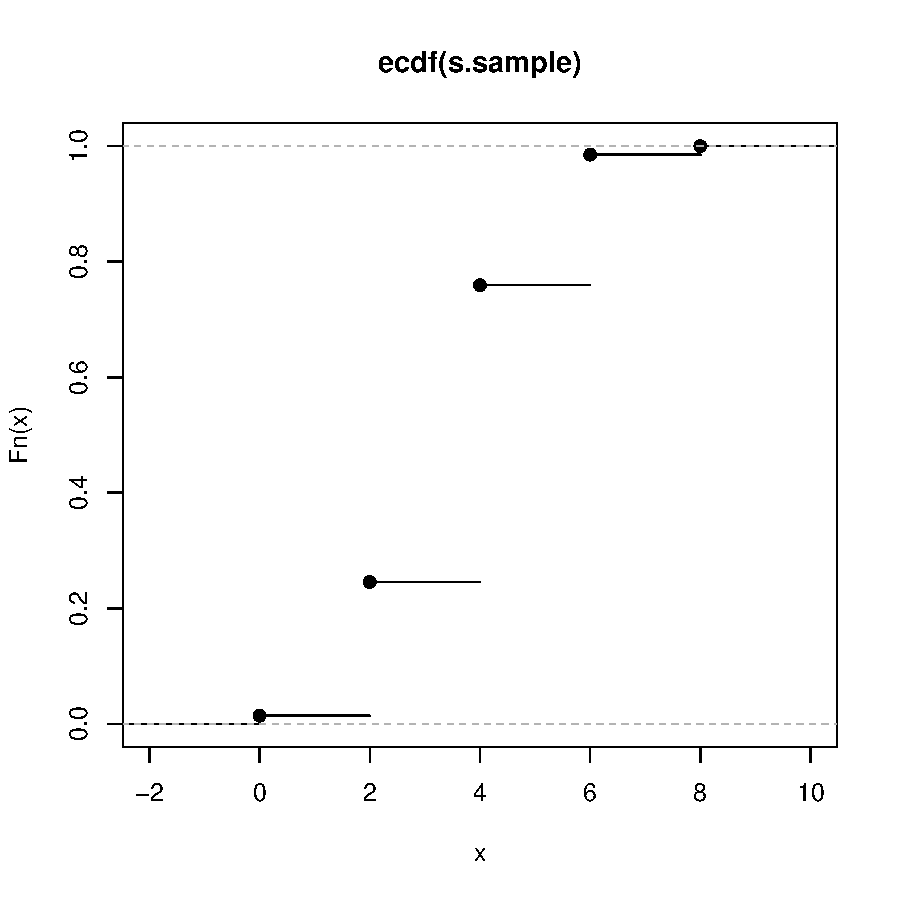
\includegraphics{fishertest-004}
\par
Notice that only even values of $S$ are possible. The jumps in the center
of the plot, around 4, are the biggest, showing that those values are more
likely.
\end{Answer}

\begin{Exercise}
Define the shape of the rejection region. Is it unilateral or bilateral?
Estimate the p-value of the test. What do we conclude?
\par\noindent\textcolor{BrickRed}{\textbf{For the aces:} If instead of
the agreed protocol, Fisher had flipped a coin to know if he would pour
tea or milk first, what would be the p-value of the test for the given
data?}
\end{Exercise}
\begin{Answer}
In that case, unilateral testing makes sense, because if Muriel guesses
extremely poorly, we'd rather conclude that she is unlucky (and not that
she has the special ability to not guess if tea or milk was first).
Then estimating the p-value is just a matter of
\begin{Schunk}
\begin{Sinput}
> mean(s.sample >= 6);
\end{Sinput}
\begin{Soutput}
[1] 0.2406
\end{Soutput}
\end{Schunk}
\end{Answer}

\begin{Exercise}
Compare the results with the output of \texttt{fisher.test}. For this
you need to create the $2\times 2$ contingency table with the function
\texttt{matrix}.
\end{Exercise}
\begin{Answer}
\begin{Schunk}
\begin{Sinput}
> contab <- matrix(c(3,1,1,3), ncol=2);
> fisher.test(contab, alternative="greater");
\end{Sinput}
\begin{Soutput}
	Fisher's Exact Test for Count Data

data:  contab 
p-value = 0.2429
alternative hypothesis: true odds ratio is greater than 1 
95 percent confidence interval:
 0.3135693       Inf 
sample estimates:
odds ratio 
  6.408309 
\end{Soutput}
\end{Schunk}
\par
For the anecdote, Fisher found the same result. Still, his daughter
later wrote that he was convinced that Muriel's claim was true.
Even legendary statisticians sometimes lose faith in statistics.
\end{Answer}

\cleardoublepage
\shipoutAnswer
\end{document}

